\documentclass[11pt,a4paper]{article}
\usepackage[T1]{fontenc}
\usepackage[utf8]{inputenc}
\usepackage{lmodern}
\usepackage{amsmath}
\usepackage{underscore}
\usepackage[margin=2.3cm]{geometry}
\usepackage{xcolor}
\usepackage{booktabs}
\usepackage{longtable}
\usepackage{array}
\usepackage{enumitem}
\usepackage{graphicx}
\usepackage{listings}
\usepackage{tikz}
\usetikzlibrary{positioning,arrows.meta,shapes.geometric,fit,calc}
\usepackage{fancyhdr}
\usepackage[hidelinks]{hyperref}

\definecolor{accent}{HTML}{6D28D9}
\definecolor{code}{HTML}{F5F5F7}
\definecolor{kw}{HTML}{0550AE}
\definecolor{cmt}{HTML}{6A737D}
\definecolor{str}{HTML}{0A7D22}
\definecolor{boxfill}{HTML}{EEF2FF}
\definecolor{boxline}{HTML}{6D28D9}
\definecolor{greyfill}{HTML}{F2F2F2}

\lstdefinestyle{py}{
  language=Python, basicstyle=\ttfamily\footnotesize, backgroundcolor=\color{code},
  keywordstyle=\color{kw}\bfseries, commentstyle=\color{cmt}\itshape,
  stringstyle=\color{str}, numbers=left, numberstyle=\tiny\color{cmt},
  breaklines=true, frame=single, rulecolor=\color{gray!40}, framesep=5pt,
  showstringspaces=false, columns=fullflexible, xleftmargin=16pt}
\lstset{style=py}
\newcommand{\code}[1]{\texttt{#1}}

\pagestyle{fancy}\fancyhf{}
\lhead{\small Wafer Map Tool --- Architecture \& Flow}
\rhead{\small\thepage}
\renewcommand{\headrulewidth}{0.4pt}

\tikzset{
  box/.style={rectangle, rounded corners=3pt, draw=boxline, fill=boxfill,
    align=center, inner sep=5pt, font=\footnotesize, minimum height=8mm},
  grey/.style={rectangle, rounded corners=3pt, draw=gray!60, fill=greyfill,
    align=center, inner sep=5pt, font=\footnotesize, minimum height=8mm},
  io/.style={rectangle, draw=gray!70, fill=white, align=center, inner sep=4pt,
    font=\scriptsize, minimum height=7mm},
  arr/.style={-{Stealth[length=2.4mm]}, thick, draw=gray!70},
}

\begin{document}

\begin{titlepage}
\centering
\vspace*{3cm}
{\Huge\bfseries Wafer Map Tool}\\[4pt]
{\Large Architecture, Data Flow \& GUI Design}\\[6pt]
{\large Technical Reference --- v2.3}\\[2cm]
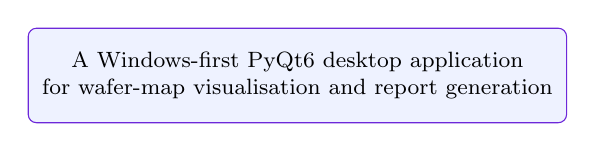
\begin{tikzpicture}
\node[box, minimum width=5cm, minimum height=1.2cm] {A Windows-first PyQt6 desktop application\\for wafer-map visualisation and report generation};
\end{tikzpicture}\\[2cm]
{\large Covers: input loading (TXT/CSV, raw \texttt{.eff}), the report pipeline,\\
the wafer-map rendering engine (interpolate / extrapolate / ``no-data'' grey),\\
the GUI shell, and the headless automation layer.}\\[1cm]
{\normalsize Generated \today}
\vfill
\end{titlepage}

\tableofcontents
\newpage

% ======================================================================
\section{Overview}
The \textbf{Wafer Map Tool} turns semiconductor wafer measurement files into
colour-coded wafer-map reports (PDF, PPTX and a CSV colour summary). It runs
as a PyQt6 desktop application and, through the same codebase, as a headless
command-line / scheduled-task runner.

\begin{center}\small
\begin{tabular}{@{}ll@{}}
\toprule
\textbf{Property} & \textbf{Value}\\
\midrule
Language / UI & Python 3.13, PyQt6 (Qt~6) \\
Numerics & NumPy, pandas, SciPy (\texttt{griddata}, \texttt{cKDTree}) \\
Rendering & Matplotlib (\texttt{Agg} backend --- non-interactive) \\
Exports & PDF (vector, \texttt{pypdf} merge), CSV, PPTX (\texttt{python-pptx}) \\
Inputs & \texttt{.txt}/\texttt{.csv} (delimited), raw \texttt{.eff} (eSquare) \\
Entry points & \texttt{main.py} (GUI), \texttt{run\_job.py} (headless) \\
Packaging & PyInstaller (\texttt{WaferMapTool.spec}); exe doubles as runner \\
\bottomrule
\end{tabular}
\end{center}

\noindent\textbf{Core idea.} A measurement file is normalised to a single
\texttt{pandas} table with columns \code{lot}, \code{wafer}, \code{x}, \code{y},
\code{value}. The pipeline groups it by (lot,~wafer), interpolates each wafer
onto a disc, colours it against two thresholds, and emits a multi-page report.

% ======================================================================
\section{System Architecture}
The code is organised by \emph{owner / helper} boundaries: the UI layer owns
interaction and preview; \code{report.py} owns pipeline orchestration;
lower-level modules are pure/stateless where possible.

\begin{center}\small
\begin{longtable}{@{}p{4.6cm}p{10.2cm}@{}}
\toprule
\textbf{Module} & \textbf{Responsibility}\\
\midrule
\endhead
\texttt{main.py} & Entry point. Routes \code{--run-job}/\code{--test-email}/bare \texttt{.wtjob} to the headless runner, else opens the GUI. \\
\texttt{wafer\_tool/config.py} & \code{PlotConfig} (shared UI$\leftrightarrow$pipeline contract), \code{ColorScheme}, tuning constants. \\
\texttt{wafer\_tool/data\_loader.py} & Read/normalise delimited TXT/CSV into the 5-column DataFrame. \\
\texttt{wafer\_tool/eff\_loader.py} & Raw \texttt{.eff} reader: header scan, per-parameter streaming extraction, spec limits, value filter. \\
\texttt{wafer\_tool/eff\_pipeline.py} & GUI-free orchestration: one report per selected \texttt{.eff} parameter. \\
\texttt{wafer\_tool/report.py} & Pipeline orchestration: load $\to$ stats $\to$ render $\to$ export. \\
\texttt{wafer\_tool/geometry.py} & Pure maths: transforms, \code{build_wafer_grid}, \code{far_from_data_mask}. \\
\texttt{wafer\_tool/plotting.py} & \code{draw_wafer_ax} --- renders one wafer map (zones, grey, outline). \\
\texttt{wafer\_tool/statistics.py} & Wafer classification and the 8-condition summary page. \\
\texttt{wafer\_tool/exporters/} & \code{pdf_exporter}, \code{csv_exporter}, \code{pptx_exporter}, \code{report_charts}. \\
\texttt{wafer\_tool/worker.py} & \code{ReportWorker} --- QThread wrapper for TXT/CSV runs. \\
\texttt{wafer\_tool/eff\_worker.py} & \code{EffReportWorker} / \code{EffPreviewWorker} --- QThreads for \texttt{.eff}. \\
\texttt{wafer\_tool/ui/main\_window.py} & \code{DataProcessorUI} --- the application shell, previews, controls. \\
\texttt{wafer\_tool/automation/} & \code{job.py} (\texttt{.wtjob} format), \code{runner.py} (headless), \code{scheduler*} (Windows Task Scheduler), \code{notify.py} (email). \\
\bottomrule
\end{longtable}
\end{center}

% ======================================================================
\section{Data Flow}
At the top level, every run funnels into \code{generate_report()}, which is the
single orchestration boundary.

\begin{figure}[h]\centering
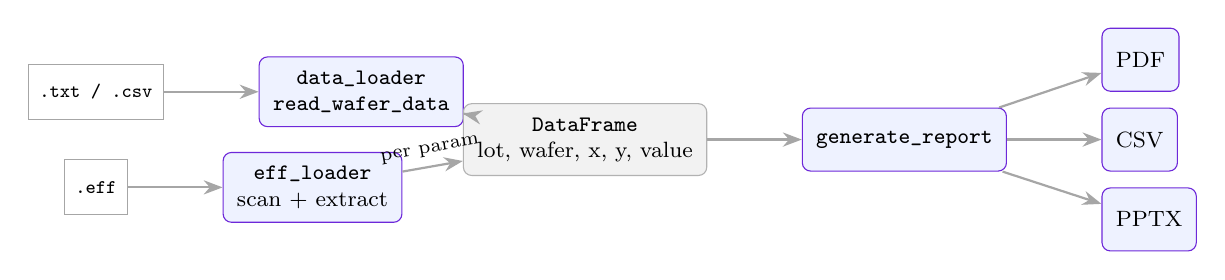
\begin{tikzpicture}[node distance=7mm and 12mm]
\node[io] (txt) {\texttt{.txt / .csv}};
\node[io, below=5mm of txt] (eff) {\texttt{.eff}};
\node[box, right=of txt] (dl) {\texttt{data\_loader}\\\code{read_wafer_data}};
\node[box, right=of eff] (el) {\texttt{eff\_loader}\\scan + extract};
\node[grey, right=16mm of $(dl)!0.5!(el)$] (df) {\texttt{DataFrame}\\lot, wafer, x, y, value};
\node[box, right=of df] (gr) {\code{generate_report}};
\node[box, above right=2mm and 12mm of gr] (pdf) {PDF};
\node[box, right=12mm of gr] (csv) {CSV};
\node[box, below right=2mm and 12mm of gr] (ppt) {PPTX};
\draw[arr] (txt)--(dl); \draw[arr] (eff)--(el);
\draw[arr] (dl)--(df); \draw[arr] (el)-- node[font=\scriptsize,sloped,above]{per param} (df);
\draw[arr] (df)--(gr);
\draw[arr] (gr)--(pdf); \draw[arr] (gr)--(csv); \draw[arr] (gr)--(ppt);
\end{tikzpicture}
\caption{Top-level data flow. Both input kinds normalise to the same DataFrame; one \texttt{.eff} yields one report per selected parameter.}
\end{figure}

\subsection{Input loading --- TXT / CSV}
\code{read_wafer_data} (in \texttt{data\_loader.py}) parses delimited text with
the fast pandas C engine, trying \textbf{tab}, then \textbf{comma}, then (last
resort) a slow whitespace regex. It accepts either:
\begin{itemize}[nosep,leftmargin=1.4em]
\item \textbf{5+ columns}: \code{lot}, \code{wafer}, \code{x}, \code{y}, \code{value}; or
\item \textbf{4 columns}: a combined \code{"LotID WaferID"} first column + \code{x}, \code{y}, \code{value}.
\end{itemize}
Identifier columns are forced to text (so \code{"01"} keeps its leading zero);
\code{x}/\code{y}/\code{value} are parsed natively to \code{float32}. Rows with
unparseable numbers are dropped. \emph{Excel (\texttt{.xls}/\texttt{.xlsx}) is
not currently handled by this path --- see \S\ref{sec:gaps}.}

\subsection{Input loading --- raw \texttt{.eff}}
An \texttt{.eff} (eSquare) file is a \texttt{;}-delimited export with a metadata
header, per-column \texttt{<...>} descriptor rows, then data rows. The loader
exposes:
\begin{itemize}[nosep,leftmargin=1.4em]
\item \code{scan_eff(path)} --- header-only scan (cheap even for GB files): detects the
\code{lot}/\code{wafer}/\code{x}/\code{y} coordinate columns and the list of
selectable \code{EffParameter}s, \emph{including each parameter's spec limits}
(\code{<LIMIT:SPEC:LOWER_VALUE>} / \code{UPPER_VALUE}).
\item \code{extract_parameters(...)} --- one streaming pass writing one
\code{lot wafer\textbackslash t x\textbackslash t y\textbackslash t value} text file per selected parameter,
into its own output folder. Supports an inclusive \textbf{value filter}
(\code{filter_min}/\code{filter_max}); positions removed by the filter are
remembered (\code{die_sites}) so the wafer outline stays full-size, and wafers
emptied by the filter are recorded (\code{empty_wafers}).
\end{itemize}
Each extracted parameter then flows through the same \code{generate_report}.

% ======================================================================
\section{Report Pipeline}
\code{generate_report(filepath, config, out_dir, \dots)} performs, in order:
\begin{enumerate}[nosep,leftmargin=1.6em]
\item \textbf{Load} data (\code{read_wafer_data}).
\item \textbf{Statistics}: \code{calculate_8_condition_statistics}.
\item \textbf{Per-wafer PNGs} (optional) --- only when a live preview is attached
(\code{on_wafer_ready}) or \code{render_individual_pngs=True}; headless runs skip
this (it was ${\sim}40\%$ of runtime).
\item \textbf{PDF} (\code{generate_pdf}): overview charts, summary, 8-condition page,
then 5$\times$5 per-lot wafer grids. Grid pages render in parallel across
processes for large reports and merge with \texttt{pypdf}.
\item \textbf{CSV} colour summary.
\item \textbf{PPTX} (if \texttt{python-pptx} present): assembled from per-page PNGs.
\end{enumerate}

\begin{figure}[h]\centering
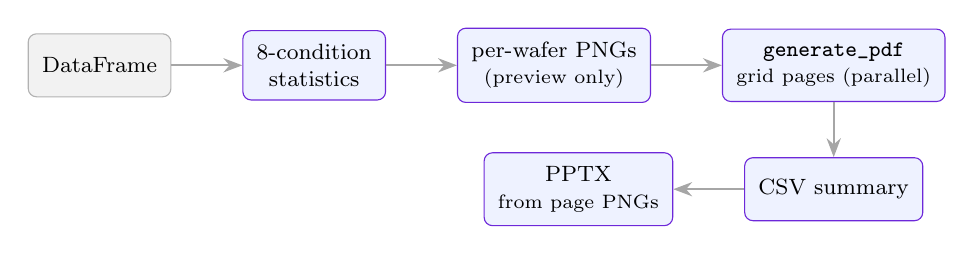
\begin{tikzpicture}[node distance=6mm and 9mm]
\node[grey] (d) {DataFrame};
\node[box, right=of d] (st) {8-condition\\statistics};
\node[box, right=of st] (pv) {per-wafer PNGs\\\scriptsize(preview only)};
\node[box, right=of pv] (pdf) {\code{generate_pdf}\\\scriptsize grid pages (parallel)};
\node[box, below=7mm of pdf] (csv) {CSV summary};
\node[box, left=of csv] (ppt) {PPTX\\\scriptsize from page PNGs};
\draw[arr] (d)--(st); \draw[arr] (st)--(pv); \draw[arr] (pv)--(pdf);
\draw[arr] (pdf)--(csv); \draw[arr] (csv)--(ppt);
\end{tikzpicture}
\caption{Report pipeline stages inside \texttt{generate\_report}.}
\end{figure}

\subsection{The two run paths (must stay in sync)}
The \emph{same} \code{generate_report} is driven two ways. Behaviour that must
happen on every run (email, run-history logging) has to be wired into
\textbf{both}.

\begin{figure}[h]\centering
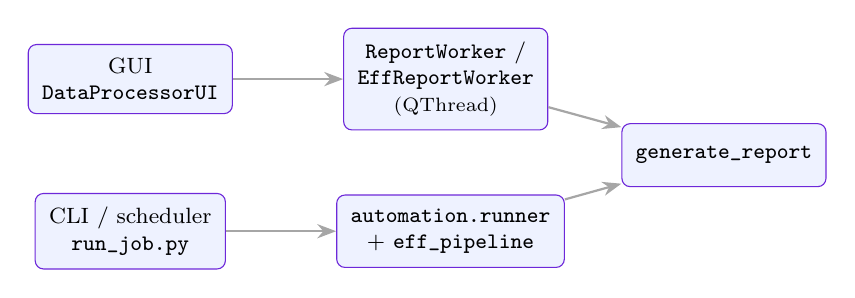
\begin{tikzpicture}[node distance=6mm and 14mm]
\node[box] (gui) {GUI\\\code{DataProcessorUI}};
\node[box, below=10mm of gui] (cli) {CLI / scheduler\\\code{run_job.py}};
\node[box, right=of gui] (rw) {\code{ReportWorker} /\\\code{EffReportWorker}\\\scriptsize(QThread)};
\node[box, right=of cli] (run) {\code{automation.runner}\\+ \code{eff_pipeline}};
\node[box, right=22mm of $(rw)!0.5!(run)$] (gr) {\code{generate_report}};
\draw[arr] (gui)--(rw); \draw[arr] (cli)--(run);
\draw[arr] (rw)--(gr); \draw[arr] (run)--(gr);
\end{tikzpicture}
\caption{GUI workers and the headless runner both converge on \texttt{generate\_report}.}
\end{figure}

% ======================================================================
\section{Wafer-Map Rendering Engine}
\label{sec:render}
A single wafer is drawn by \code{draw_wafer_ax(ax, df, wafer_id, config,
lot_sites=\dots)}. The geometry is built once, then two user options decide how
gaps are handled.

\subsection{Grid construction (\texttt{geometry.build\_wafer\_grid})}
\begin{enumerate}[nosep,leftmargin=1.6em]
\item Lay a $100\times100$ mesh over the wafer disc (centre + radius from the
\emph{lot} die extent, so every wafer of a lot shares one outline).
\item \textbf{Linear} \code{griddata} interpolates measured values between dies
(NaN outside the convex hull).
\item \textbf{Nearest-neighbour} \code{griddata} fills the remaining NaN holes
(this is the ``extension''), then values are clamped to $[z_{\min},z_{\max}]$.
\item Cells outside the wafer circle are masked to NaN.
\end{enumerate}

\subsection{Interpolate vs.\ Extrapolate, and the ``no-data'' grey}
\code{far_from_data_mask} (a \code{cKDTree} query) flags grid cells whose nearest
measured die is farther than \code{MAX_INTERP_DIST_CHIPS} $\times$
\code{DIE_PITCH} ($=4$ chips). The render then branches on two
\code{PlotConfig} flags:

\begin{center}\small
\begin{tabular}{@{}lll@{}}
\toprule
\textbf{Mode} & \texttt{extrapolate} & \textbf{Effect} \\
\midrule
Interpolate & \code{False} & Colour only within 4 chips of a die; farther cells are ``no data''. \\
Extrapolate & \code{True} & Keep the nearest-fill everywhere --- the whole disc is coloured. \\
\bottomrule
\end{tabular}\\[4pt]
\begin{tabular}{@{}lll@{}}
\toprule
\textbf{} & \texttt{show\_missing\_grey} & \textbf{Effect on ``no-data'' cells (Interpolate only)} \\
\midrule
Grey on & \code{True} & Painted grey (\code{COLOR_MISSING}); ``No data'' legend entry. \\
Grey off & \code{False} & Left blank/white (wafer outline still drawn). \\
\bottomrule
\end{tabular}
\end{center}

\begin{lstlisting}[caption={The interpolate/extrapolate + grey decision in draw\_wafer\_ax.}]
if config.extrapolate:
    missing = None                       # keep the full nearest-fill
else:
    missing = (far_from_data_mask(xi, yi, x, y,
                                  MAX_INTERP_DIST_CHIPS * DIE_PITCH)
               & ~np.isnan(zi))          # cells > 4 chips from any die

if missing is not None:
    zi[missing] = np.nan                 # drop "no data" cells from the fill
# ... contourf the three threshold zones (low / mid / high) ...
if missing is not None and config.show_missing_grey:
    ax.contourf(xi, yi, np.where(missing, 1.0, np.nan),
                levels=[0.5, 1.5], colors=[COLOR_MISSING])   # grey overlay
# wafer outline (neutral grey, visible on any background)
ax.add_patch(Circle((x_mid, y_mid), radius, fill=False,
                    color="#888888", linewidth=1.0))
\end{lstlisting}

\begin{figure}[h]\centering
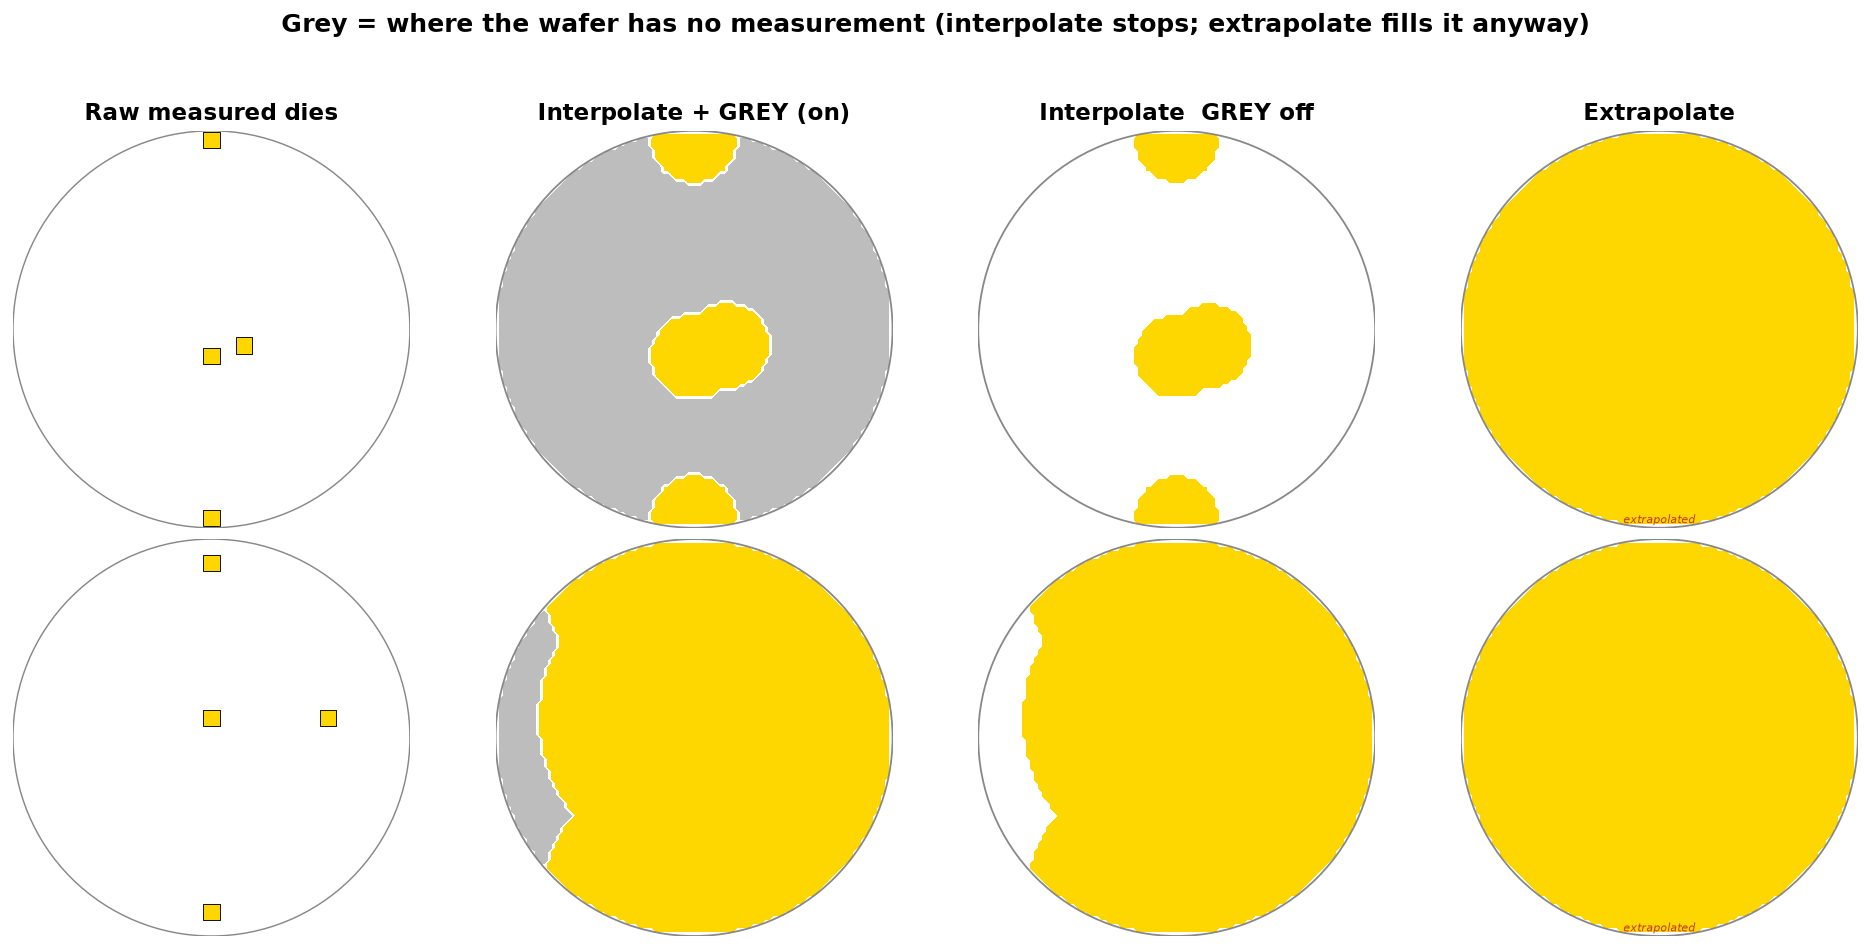
\includegraphics[width=\linewidth]{grey_demo.png}
\caption{Two sparsely-sampled wafers (4 of 10 sites). \textbf{Grey = where there is
no measurement.} Left$\to$right: raw dies; interpolate with grey on; same with
grey off (blank); extrapolate (whole wafer filled from the nearest readings).}
\end{figure}

\noindent\textbf{Colouring.} Values map to three zones against the two
thresholds ($t_{\text{low}}$, $t_{\text{high}}$) via a \code{contourf} with the
run's \code{ColorScheme} (\emph{Reverse / High=Green} swaps low$\leftrightarrow$high
colours). \code{use_log} applies a $\log_{10}$ mapping (magnitudes clamped to
avoid $\log 0$). Spatial \code{mirror_x}/\code{mirror_y}/\code{rot_deg} transforms
are applied before gridding. \emph{All $256$ combinations of these options were
exercised without error (\S\ref{sec:test}).}

% ======================================================================
\section{Configuration Contract}
\code{PlotConfig} is the single typed object passed from UI state into the
pipeline and the renderer.

\begin{center}\small
\begin{tabular}{@{}lll@{}}
\toprule
\textbf{Field} & \textbf{Type} & \textbf{Meaning}\\
\midrule
\code{t_low}, \code{t_high} & float & Lower/upper thresholds (normalised low$\le$high). \\
\code{use_log} & bool & $\log_{10}$ value mapping. \\
\code{high_is_green} & bool & Reverse the zone colours (high = green). \\
\code{mirror_x}, \code{mirror_y} & bool & Spatial mirror. \\
\code{rot_deg} & int & Clockwise rotation $\in\{0,90,180,270\}$. \\
\code{show_missing_grey} & bool & \textbf{(new)} Grey the ``no-data'' areas vs.\ blank. \\
\code{extrapolate} & bool & \textbf{(new)} Fill whole wafer vs.\ interpolate-near-dies. \\
\bottomrule
\end{tabular}
\end{center}

\noindent Key tuning constants (\texttt{config.py}):
\code{GRID_RESOLUTION=100}, \code{DIE_PITCH=1.0},
\code{MAX_INTERP_DIST_CHIPS=4}, \code{MIN_POINTS_FOR_PLOT=4},
\code{MAX_WAFERS_PER_PAGE=25}, \code{PAGE_PNG_DPI=110},
\code{WAFER_PNG_DPI_UNIFORM=70}, \code{WAFER_PNG_DPI_MULTIZONE=150},
\code{COLOR_MISSING} (grey, \#BDBDBD).

% ======================================================================
\section{GUI Architecture}
\code{DataProcessorUI} (a \code{QMainWindow}) splits into a \textbf{left control
panel} (now inside a \code{QScrollArea}, so controls never overlap on short
windows) and a \textbf{right preview panel} with tabs.

\begin{figure}[h]\centering
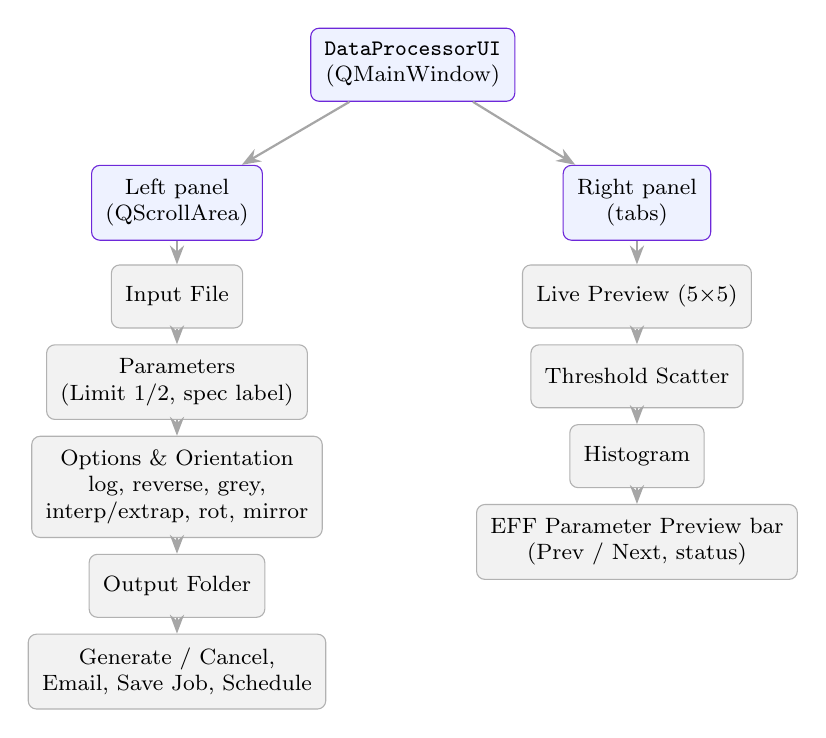
\begin{tikzpicture}[node distance=4mm and 8mm, every node/.style={font=\scriptsize}]
\node[box] (root) {\code{DataProcessorUI}\\(QMainWindow)};
\node[box, below left=8mm and 6mm of root] (left) {Left panel\\(QScrollArea)};
\node[box, below right=8mm and 6mm of root] (right) {Right panel\\(tabs)};
\node[grey, below=3mm of left] (g1) {Input File};
\node[grey, below=2mm of g1] (g2) {Parameters\\(Limit 1/2, spec label)};
\node[grey, below=2mm of g2] (g3) {Options \& Orientation\\log, reverse, grey,\\interp/extrap, rot, mirror};
\node[grey, below=2mm of g3] (g4) {Output Folder};
\node[grey, below=2mm of g4] (g5) {Generate / Cancel,\\Email, Save Job, Schedule};
\node[grey, below=3mm of right] (t1) {Live Preview (5$\times$5)};
\node[grey, below=2mm of t1] (t2) {Threshold Scatter};
\node[grey, below=2mm of t2] (t3) {Histogram};
\node[grey, below=2mm of t3] (t4) {EFF Parameter Preview bar\\(Prev / Next, status)};
\draw[arr] (root)--(left); \draw[arr] (root)--(right);
\draw[arr] (left)--(g1);\draw[arr] (g1)--(g2);\draw[arr](g2)--(g3);\draw[arr](g3)--(g4);\draw[arr](g4)--(g5);
\draw[arr] (right)--(t1);\draw[arr](t1)--(t2);\draw[arr](t2)--(t3);\draw[arr](t3)--(t4);
\end{tikzpicture}
\caption{GUI widget tree. The \emph{Options \& Orientation} group hosts the new grey / interpolate / extrapolate controls.}
\end{figure}

\subsection{Background workers \& signals}
Heavy work never runs on the UI thread. Three \code{QThread}s:
\begin{itemize}[nosep,leftmargin=1.4em]
\item \code{ReportWorker} --- TXT/CSV report. Signals: \code{progress},
\code{wafer_progress}, \code{status_message}, \code{wafer_ready},
\code{report_done}, \code{error}.
\item \code{EffReportWorker} --- one report per selected \texttt{.eff} parameter
(wraps \code{eff_pipeline.process_eff}). Adds \code{param_done} / \code{all_done}.
\item \code{EffPreviewWorker} --- reads one parameter in the background to feed the
scatter/histogram preview without blocking the UI.
\end{itemize}
Cancellation is cooperative (a \code{threading.Event} checked between wafers).
The \textbf{wafer-map options} (\S\ref{sec:render}) are read from the Options
group into a \code{PlotConfig} at launch (both the TXT and \texttt{.eff} run
handlers), and persisted into saved \texttt{.wtjob}s via \code{_PLOT_KEYS}.

\subsection{Live preview vs.\ report}
The \emph{Threshold Scatter} and \emph{Histogram} tabs are value-distribution
views (no wafer geometry); the grey / interpolate / extrapolate options do
\emph{not} affect them. Those options change the \emph{wafer maps} --- the
\emph{Live Preview (5$\times$5)} grid (filled as wafers render) and the PDF/PPTX.

% ======================================================================
\section{Automation \& Scheduling}
A run can be saved as a \texttt{.wtjob} (JSON) capturing the input, output
folder and every \code{PlotConfig} field (now including \code{show_missing_grey}
and \code{extrapolate}), plus \texttt{.eff} parameter selection, the value
filter, and email settings.
\begin{itemize}[nosep,leftmargin=1.4em]
\item \code{run_job.py <job.wtjob>} replays a job headlessly via
\code{automation.runner.main}.
\item \code{scheduler.py} / \code{scheduler_dialog.py} register jobs with Windows
Task Scheduler; the frozen \texttt{WaferMapTool.exe} is invoked as
\code{WaferMapTool.exe --run-job <job>}.
\item \code{notify.py} optionally emails links (PDF / PPTX / output folder) via
Outlook COM or SMTP (credentials from environment variables).
\item Every run appends a row to \texttt{run\_history.csv}; the general log is
\texttt{wafer\_tool.log}. Both writes are non-fatal.
\end{itemize}

% ======================================================================
\section{Validation \& Testing}
\label{sec:test}
The current build was exercised as follows.

\begin{center}\small
\begin{tabular}{@{}p{6.4cm}p{8.2cm}@{}}
\toprule
\textbf{Check} & \textbf{Result}\\
\midrule
Full pipeline on \textbf{all 6} \texttt{.eff} files, both modes (real \code{generate_report}: PDF+CSV+PPTX) & \textbf{PASS} --- 6/6 interpolate, 6/6 extrapolate; valid multi-page PDFs. \\
Render-option combinations (\texttt{extrapolate}$\times$\texttt{grey}$\times$\texttt{log}$\times$\texttt{reverse}$\times$\texttt{mirror}$\times$\texttt{rotation}) & \textbf{768/768 OK}, 0 crashes (across dense, sparse and all-zero wafers). \\
Automation unit tests (\code{test_automation.py}) & \textbf{18/18 passed}. \\
\bottomrule
\end{tabular}
\end{center}

% ======================================================================
\section{Recent Changes \& Known Gaps}\label{sec:gaps}
\textbf{Added in this cycle:}
\begin{itemize}[nosep,leftmargin=1.4em]
\item ``\emph{Show missing data in grey}'' checkbox and an \emph{Interpolate /
Extrapolate} choice (new \code{PlotConfig} fields, honoured by the renderer and
both run paths, persisted in \texttt{.wtjob}s).
\item Wafer outline drawn in neutral grey so it is visible on any background
(previously white $\Rightarrow$ invisible on the white report background).
\item Left control panel wrapped in a scroll area (fixes Rotation/Mirror
crowding on short windows).
\end{itemize}

\textbf{Known gaps (candidates for the next cycle):}
\begin{itemize}[nosep,leftmargin=1.4em]
\item \textbf{Excel import}: \texttt{.xls}/\texttt{.xlsx} are \emph{not} read by
\code{data_loader} (CSV/TXT only). Adding \code{pd.read_excel} + a file-dialog
filter would close this.
\item \textbf{Value filter for TXT/CSV}: the inclusive value filter exists only
on the \texttt{.eff} path; TXT/CSV imports are unfiltered.
\end{itemize}

\vfill
\noindent\rule{\linewidth}{0.4pt}\\
{\footnotesize This document reflects the source as of the stated date. Where
the README and the code disagree, the code is authoritative.}

\end{document}
